%форматирование размера документа
\documentclass[11pt, a4paper]{article}

\usepackage{geometry}
% total - determines printable width, height
\geometry{ 
	a4paper, total={160mm,267mm}
}
\columnsep 10mm
\usepackage{fancyhdr}
\pagestyle{fancy}

% colontituls 
\renewcommand{\headrulewidth}{0 pt}
\cfoot{}
\footskip=5mm

%----text,fonts------------------------------------------------------------------------------------
\usepackage{mmap}
\usepackage[T2A]{fontenc}
\usepackage[utf8]{inputenc}
\usepackage[english, russian]{babel}
\usepackage{setspace}
\setstretch{0,9}

%----math,graphics---------------------------------------------------------------------------------
\usepackage{amsmath,amsfonts,amssymb}
\usepackage{amsthm}
\usepackage{listings}

\usepackage{tikz}
\usetikzlibrary{calc}
\usepackage{pgfplots}
\pgfplotsset{
	compat=1.17
}

\usepackage{graphicx}
\graphicspath{{image/}}

\usepackage{wrapfig}
\usepackage{tabularx}

% relative importing
\usepackage{import}

\begin{document}

\import{}{titular.tex}
\newpage

\section{Описание метода. Расчетные формулы}

Метод Симпсона -- частный случай формул Ньютона-Котеса при $k = 2$. То есть пусть требуется найти 
вычислить интеграл 
\[
y = \int_a^b f(x)
\]

выбрав шаг 
\[
  h = \dfrac{b - a}{n}
\]
Тогда разобьем отрезок с помощью равноотстоящих точек $x_i = a + h * i$ на n равных частей.

Заменяя функцию $y_i = f(x_i)$ интерполяционным полиномом Лагранжа, который позволяет через 
заданное количество точек провести кривую получим приближенную квадратурную формулу.
\[
  \int_{x_0}^{x_n} y dx = \sum_{i = 0}^{n} A_i y_i
\]

Теперь если в эту формулу добавить постоянные коэффициенты Котеса, об этом рассказано в Демидовиче, то получим 
формулу
\[
  \int_{a}^b y dx = (b-a) * \sum_{i = 0}^n H_i y_i
\], 
где $H_i$ - коэффициент Котеса.

А теперь, если в этой формуле принять $n = 2$, то получим формулу Симпсона для нахождения 
значения интеграла функции. Коротко, мы разделяем отрезок $[a, b]$ на $n$ частей и проводим
через них параболы. 

То есть формула для 3-х точек будет выглядеть следующим образом  
\[
  \int_{x_0}^{x^n} y dx = \dfrac{h}{3} * (y_0 + 4 * y_1 + y_2)
\]
\medskip

Теперь рассмотрим общий случай. Пусть $n = 2*m$ четное число и $f(x_i)$ $(i = 0, 1, 2, \ldots, n)$ - значения функций в точках.
Сами точки являются равноотстоящими и определяются по формуле, указанной выше. Тогда применяя 
формулу к удвоенному промежутку $[x_0 x_2], [x_2 x_4] \\ \ldots [x_{n-2} x_n]$ будем иметь.

\begin{equation*}
  \int_a^b y dx = \dfrac{h}{3} (y_0 + 4y_1 + y_2) + \dfrac{h}{3} (y_2 + 4y_3 + y_4) + \ldots
  + \dfrac{h}{3} (y_{n-2} + 4y_{n-1} + y_n) 
\end{equation*}

Введя обозначения 
\begin{equation*}
  \sigma_1 = y_1 + y_3 + \ldots + y_{n-1}

  \sigma_2 = y_2 + y_4 + \ldots + y_n
\end{equation*}

запишем формулу в укороченном виде:

\begin{equation*}
  \int_a^b y dx = \dfrac{h}{3} [(y_0 + y_n) + 4 \sigma_1 + 2 \sigma_2)]
\end{equation*}


\section{Блок схема численного метода.}

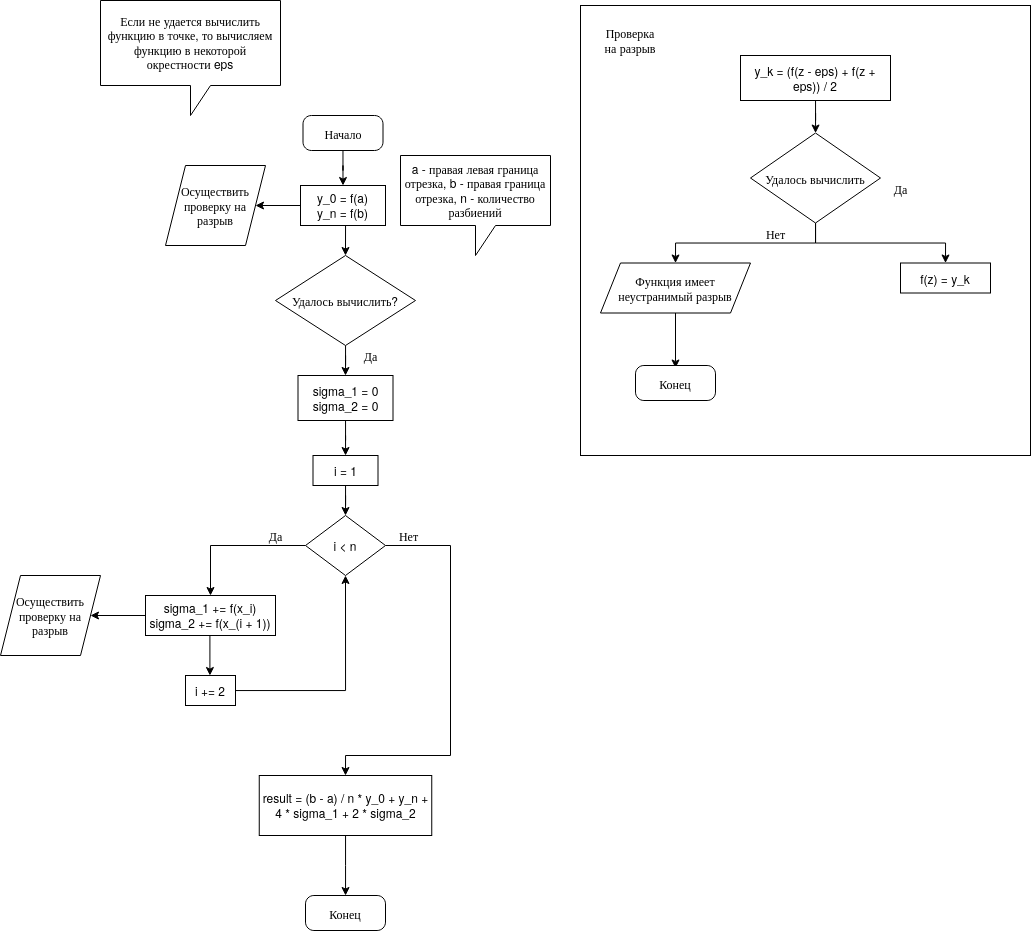
\includegraphics[width=\linewidth]{draw.png}

\section{Листинг реализованного численного метода.}

\begin{verbatim}
  y0 = calculate(equation, {var_lst[0]: range_min})
  yn = calculate(equation, {var_lst[0]: range_max})
  n = int((range_max - range_min) / step)

  sigma1 = sum([calculate(
    equation, {var_lst[0]: range_min + step * i}) for i in range(1, n, 2)])
  sigma2 = sum([calculate(
    equation, {var_lst[0]: range_min + step * i}) for i in range(2, n, 2)])

  return (step / 3) * (y0 + yn + 4 * sigma1 + 2 * sigma2)
\end{verbatim}

\section{Примеры и результаты работы программы на разных данных.}


\section{Вывод.}
\end{document}
